% Metódy inžinierskej práce

\documentclass[10pt,twoside,slovak,a4paper]{article} 

\usepackage[slovak]{babel}
%\usepackage[T1]{fontenc}
\usepackage[IL2]{fontenc} % lepšia sadzba písmena Ľ než v T1
\usepackage[utf8]{inputenc}
\usepackage{graphicx}
\usepackage{url} % príkaz \url na formátovanie URL
\usepackage{hyperref} % odkazy v texte budú aktívne (pri niektorých triedach dokumentov spôsobuje posun textu)
\graphicspath{{./images/}}
\usepackage{cite}


\pagestyle{headings}

\title{Ako vyhľadávajú Google Maps\thanks{Semestrálny projekt v predmete Metódy inžinierskej práce, ak. rok 2023/24, vedenie: Vladimír Mlynarovič}} % meno a priezvisko vyučujúceho na cvičeniach

\author{Adrián Maslák\\[2pt]
	{\small Slovenská technická univerzita v Bratislave}\\
	{\small Fakulta informatiky a informačných technológií}\\
	{\small \texttt{xmaslaka@stuba.sk}}
	}

\date{\small 5. November 2023} % upravte



\begin{document}

\maketitle

\begin{abstract}
Google Maps je sofistikovaný systém máp priamo v naších zariadeniach ktorý nám umožňuje nájsť nové miesta, získať pokyny na prepravu z bodu A do bodu B. Pomôcka ktorú každodenne používa viac než miliarda používateľov.
	Aplikácia Google Maps je písaná v jazykoch C++, JavaScript, XML a AJAX.  Na vypočítanie najkratšej trasy sú použíté dva algoritmy, Dijkstrov algoritmus a A* algoritmus ktoré sú najrýchlejšie a najefektívnejšie pri hľadaní najkratšej trasy v grafoch, kde si môžeme cesty predstaviť ako jeden graf. Do týchto vyhľadavaní zasahujú aj reálne faktory ako hustota premávky alebo počasie. Vďaka dlhému vývoju nám táto aplikácia umožnuje nájsť aj alternatívne trasy a všetky dopravné obmedzenia.
	Článok končí objasnením fungovania tohto komplexného systémum, spresnením využitých funkcií a algoritmov.

Témou tohto článku je vyhľadávanie Google Maps. Google maps je každodenná pomôcka miliónov používateľov a preto treba objasniť ako to celé vlastne funguje. Pod pojmom fungovania máme na mysli systém vďaka ktorému môžeme využívať náš prenosný atlas, ktorý nás dostane z bodu A do bodu B. Celkovo sa článok zameriáva na vyhľadávacie algoritmy ale aj na vplyv premávky a udalostí v reálnom čase na vyhľadanie najkratšej, najrýchlejšej a najefektívnejšej trasy. Z pohľadu laika možno sa to zdá ako zanedbateľná vec, ale pre obecenstvo s technickým zameraním to je komplexné riešenie ktoré zahrňuje enormné množstvo úsila, pozornosti a logického myslenia. 
\end{abstract}



\section{Úvod}

Google Mapy sú jednou z najvačších inovácií v histórií technológie. Príchod tejto aplikácie od giganta v technologickom svete Google Inc. Google Mapy umožňujú používateľom hľadať najkratšie a najefektívnejšie trasy do ich destinácie. Google Mapy získali takmer 70 miliónov používateľov. Postupom času boli pridané mnohé funkcie okrem navigácie. Technológia a algoritmy použité v tomto systéme sú veľmi pokročilé. Google uchovávava a analyzuje nespočetné množstvo dát vrátane historických údajov a údajov ktoré prebiehajú v reálnom čase, to je čo robí Google Mapy neskutočne progresívne a presné.


Uveďte explicitne štruktúru článku. Tu je nejaký príklad.

Základný problém, ktorý bol naznačený v úvode, je podrobnejšie vysvetlený v časti~\ref{algoritmy}.
Dôležité súvislosti sú uvedené v častiach~\ref{dolezita} a~\ref{dolezitejsia}.
Záverečné poznámky prináša časť~\ref{zaver}.

\section{Google Maps: Používané techniky a algoritmy}
\subsection{Dijikstrov algoritmus}
Je to veľmi efektívny algoritmus vynájdený Edsger W. Dijkstrom v roku 1956. Tento algoritmus sa používa pri hľadaní najkratšej trasy medzi bodmi v ohodnotených grafoch.
\begin{figure} 
 \centering
 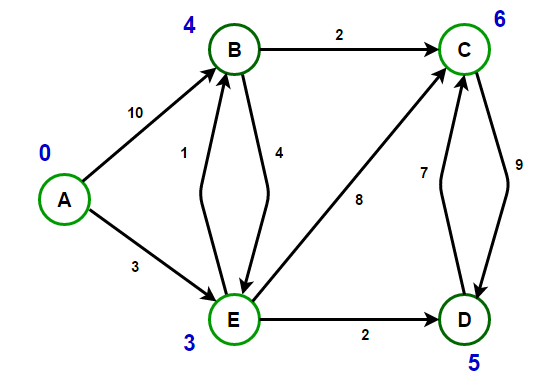
\includegraphics[width=6cm]{dijkstra}
\caption{Dijkstrov Algoritmus}

\end{figure}

Google Mapy zapájajú grafové dátové štruktúry na výpočet najkratšej trasy zo zdroja (bod A) do cieľovej destinácie (bod B). Grafová analýza obsahuje mnoho bodov a hrán cez ktoré tento algoritmus putuje a nachádza najkratšiu trasu. Aj keď je tento algoritmus jeden z najpopulárnejších, enormné množstvo bodov a hrán môže zapríčiniť zlyhanie v dôsledku predĺženia času alebo nedostatku pamäte. Drastické zväčšovanie grafu limituje efektivitu algoritmu.

\subsection{A* algoritmus}
A* Algogoritmus je flexibilný, viac efektívny. Tento algoritmus patrí do skupiny heuristických \ref{heuristika} algoritmov.
Google Mapy ho momentálne používajú na hľadanie najkratšej trasy. Dokáže prijať väčšie grafy, čo je výhoda oproti Dijkstrovmu algoritmu. A* algoritmus je široko používaný algoritmus, keďže používa a kombinuje informácie z iných algoritmov.

\begin{figure}
  \centering
  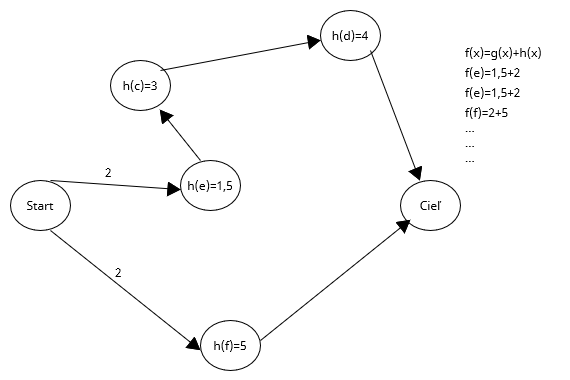
\includegraphics[width=8cm]{a-star}
  \caption{A* Algoritmus}
\end{figure}
	\begin{itemize}
	\item g(x):- Hodnota hrany medzi dvoma bodmi.
	\item h(x):- Odhadovaná hodnota do cieľa z bodu n. - Heuristická časť algoritmu.
	\item f(x):- Celková vyčíslená hodnota každého bodu.
	\end{itemize}

Celková váha vypočítaná algoritmom by nemala byť preceňovaná, keďže ide o heuristický algoritmus. Teda váha grafu, cesta po hranách z bodu A do bodu B má byť rovná alebo vačšia ako odhad váhy grafu. Narozdiel od iných algorirtmov sa tento zaoberá priamo na cieľovú destináciu (bod B). Zvyšné body a hrany neberie do úvahy. Taktiež berie do úvahy parametre ako časové požiadavky, vzdialenosť, optimalizáciu a vyberanie lepšej trasy. 




\section{Analýza cestnej premávky} 
Google Mapy narozdiel od iných GPS a navigačných systémov používajú aktuálne dáta. Čo umožnuje vyberať rýchlejšie trasy, vyhnúť sa dopravným obmedzeniam. 
Google Mapy analyzujú cestnú premávku kombinácou aktuálnych dát od používateľov a historických vzorov dopravnej situácie. Tieto dáta umožňujú predpovedať aktuálnu dopravnú situáciu ale aj blízku budúcnosť. Machine learning techniky ako grafové neurónové siete tieto predpovede spresňujú. Google Mapy taktiež zvažujú použitie smerodajných údajov od miestnych samospráv za účelom zlepšiť predpovede na základe dopravných podmienok ako stav cesty, maximálna povolená rýchlosť alebo nehodovosť určitých úsekov. Tieto rôznorodé dáta umožňujú odporúčiť najefektívnejšiu cestu ako aj predpovedať dopravné podmienky.
\subsection{Predpoveď dopravnej situácie}
Aplikácia zbiera dáta počas používania. Toto umožňuje aplikácií pochopiť aktuálnu dopravnú situáciu na cestách po celom svete. Síce tieto dáta umožnujú zistiť aktuálne predpoklady - či nás dopravná zápcha obmedzí alebo nie- nedokážu predpokladať aká bude situácia za 10, 20 alebo aj 50 minút v našej ceste. 
Aktuálne dáta o premávke v mapách sú odvodené zo súhrnu dát užívateľov používajucich aplikáciu. Tieto údaje slúžia na vizualizáciu premávky po celom svete v reálnom čase. Na predpoveď premávky, Google používa historické údaje kombinované s aktuálnymi s využitím neurónových sietí. Tento proces slúži na presné generovanie odporúčaných alebo viac efektívnych trás alebo predpovede predpokladaného príchodu.
\subsection{Detekovanie vzorov v doprave}
Google Mapy predikujú dopravu zapájaním algoritmov na spracovanie historických dát. Celý proces začína zbieraním enormného množstva anonymizovaných dát zo zariadení používateľov. Sofistikované algoritmy analyzujú tieto dáta na detekovanie bežných vzorov v doprave, ako napríklad ranné zápchy. Tieto vzory sú kritické pre predikčné modely ktoré odhadujú ako sa premávka bude správať v budúcnosti.
Avšak, nie vždy je premávka konzistentá. Google Mapy taktiež identifikujú anomálie v premávke- nezvyčajné udalosti ako dopravné nehody alebo cestné uzávierky- učí sa z nich, aby vylepšilo presnosť svojich predikcií. Počas vývinu premávky sa tieto predikčné modely menia, zapájajú najaktuálnejšie dáta na zaistenie presnosti a spoľahlivosti predikcií. Tento neustály proces učenia a adaptácie je rozhodujúci pre poskytovanie najefektívnejších a najpresnejších navigačných pokynov používateľom.



\begin{figure*}[tbh]
\centering
%\includegraphics[scale=1.0]{diagram.pdf}
Aj text môže byť prezentovaný ako obrázok. Stane sa z neho označný plávajúci objekt. Po vytvorení diagramu zrušte znak \texttt{\%} pred príkazom \verb|\includegraphics| označte tento riadok ako komentár (tiež pomocou znaku \texttt{\%}).
\caption{Rozhodujúci argument.}
\label{f:rozhod}
\end{figure*}
\section{Adaptácia k zmenám v doprave}


\section{Predpokladaný príchod}
\section{Heuristický algoritmus} \label{heuristika}
Heuristické algoritmy sú základom riešenia výpočtových problémov, najmä pri riešení zložitých problémov, kde su klasické metódy nepraktické z dôvodu časových alebo výpočtových obmedzení.
Pojem \paragraph{heuristika} pochádza z gréckeho slova /grecke slovo/ - čo v preklade znamená nájst, objaviť. Táto metóda spočíva v približnom riešení problémov. Prvý odhad sa postupom času zlepšuje na základe predošlých skúseností. Tento postup je schopný v niektorých prípadoch priniesť výsledok, aj keď neprebral všetky možnosti. Výsledok je spravidla vyjadrený dvoma spôsobmi. Buď ako kladný výsledok (odpoveď) alebo ako výrok neurčitosti. 



\section{Záver} \label{zaver} % prípadne iný variant názvu
\cite{Heuristika}
\cite{AI-and-traffic}
\cite{Djikstra's}
\cite{Algoritmy}
\cite{Heuristika2}
\cite{Algoritmy2}

Dočasné riešenie citácií...


%\acknowledgement{Ak niekomu chcete poďakovať\ldots}


% týmto sa generuje zoznam literatúry z obsahu súboru literatura.bib podľa toho, na čo sa v článku odkazujete
\bibliography{literatura}
\bibliographystyle{abbrv} % prípadne alpha, abbrv alebo hociktorý iný
\end{document}
